\documentclass[10pt]{article}

\usepackage[margin=0.75in]{geometry}
\usepackage{amsmath,amsthm,amssymb}
\usepackage{xcolor}
\usepackage{cancel}
\usepackage{graphicx}
\usepackage{changepage}
\usepackage{circuitikz}
\usepackage{pgfplots}
\usepackage{subcaption}
\usepackage{physics}
\usepackage{siunitx}
\usepackage{minted}
\usepackage[breakable]{tcolorbox}
\usepackage[inline]{enumitem}

\theoremstyle{definition}
\newtheorem{problem}{Problem}
\newtheorem{soln}{Solution}

\pgfplotsset{compat=newest}
\usetikzlibrary{lindenmayersystems}
\usetikzlibrary{arrows}

\definecolor{incolor}{HTML}{303F9F}
\definecolor{outcolor}{HTML}{D84315}
\definecolor{cellborder}{HTML}{CFCFCF}
\definecolor{cellbackground}{HTML}{F7F7F7}
\newcommand{\eq}{=}
\tikzset
{%
  axes/.style={thick,-latex},
  cylinder/.style={right color=blue!80,left color=white,fill opacity=0.7},
  paraboloid back/.style={left color=magenta!80,fill opacity=0.4},
  paraboloid front/.style={left color=white, right color=magenta!80,fill opacity=0.4},
}       

\makeatletter
\newcommand{\boxspacing}{\kern\kvtcb@left@rule\kern\kvtcb@boxsep}
\makeatother
\newcommand{\prompt}[4]{
    \ttfamily\llap{{\color{#2}[#3]:\hspace{3pt}#4}}\vspace{-\baselineskip}
}

\newcommand{\highlight}[1]{\colorbox{yellow}{$\displaystyle #1$}}

\NewDocumentCommand{\evalat}{sO{\big}mm}{%
  \IfBooleanTF{#1}
   {\mleft. #3 \mright|_{#4}}
   {#3#2|_{#4}}%
}

\title{Physics 2130: Assignment II}
\author{Jeremy Favro}
\date{\today}

\begin{document}

\maketitle

% PROBLEM 1
\begin{problem}
A particle of charge $q$ enters with a velocity $\vec{v}$ a region of space where there are both an electric, $\vec{E}$, and a magnetic field, $\vec{B}$.
It therefore experiences Lorentz electric and magnetic force, which is given by:
$$\vec{F}_L=q\left(\vec{E}+\vec{v}\cross\vec{B}\right)$$
The magnetic field, $\vec{B}$, is oriented along the $z$-axis, whilst the electric field, $\vec{E}$, lies in the $yz$-plane:
$$\vec{B}=B_z\vec{k}$$
$$\vec{E}=E_y\vec{j}+E_z\vec{k}$$
\end{problem}
\begin{soln} I'm setting an origin, not that it really matters here until we're getting constants, such that $x_0,y_0,z_0=0$
      a) b) c) d) (Sorry, I only read question a and interpreted it as find $x,y,z(t)$)
      \begin{align*}
             & \vec{F} = q\left(\vec{E}+\vec{v}\cross\vec{B}\right)                                               \\
             & \vec{F} = q\left(\vec{E}+               \begin{vmatrix}
                                                             i   & j   & k   \\
                                                             v_x & v_y & v_z \\
                                                             B_x & B_y & B_z
                                                       \end{vmatrix}\right)                                       \\
             & \vec{F} = q\left(\vec{E}+\begin{vmatrix}
                                              i   & j   & k   \\
                                              v_x & v_y & v_z \\
                                              0   & 0   & B_z
                                        \end{vmatrix}\right)                                                      \\
             & \vec{F} = q\left(\vec{E}+\left\langle v_yB_z\vec{i}-v_xB_z\vec{j} + 0\vec{k} \right\rangle \right)
      \end{align*}
      Then, using Newton's equations
      \begin{align}
             & F_x=m\ddot{x}=qB\dot{y} \rightsquigarrow E_x=0 \\
             & F_y=m\ddot{y}=qE_y-qB\dot{x}                   \\
             & F_z=m\ddot{z}=E_z
      \end{align}
      (3) can be integrated twice to obtain $$z(t)=\frac{E_z}{2m}t^2+v_{z0}t+z_0$$
      Then, simplifying (1) and (2) a bit ($\alpha\equiv \displaystyle\frac{qB}{m}$) and differentiating both we obtain
      $$\dddot{x}=\alpha\ddot{y}$$
      $$\dddot{y}=-\alpha\ddot{x}$$
      Which means that
      $$\dddot{x}=\frac{q^2BE_y}{m^2}-\alpha^2\dot{x}=\alpha^2\frac{E_y}{B}-\alpha^2\dot{x}$$
      $$\dddot{y}=-\alpha^2\dot{y}$$
      Starting with $x$
      \begin{align*}
             & \dddot{x}=\alpha^2\frac{E_y}{B}-\alpha^2\dot{x} \\
             & \ddot{v_x}=\alpha^2\frac{E_y}{B}-\alpha^2v_x    \\
             & \ddot{v_x}+\alpha^2v_x=\alpha^2\frac{E_y}{B}
      \end{align*}
      Which has a solution of the form $v_x=v_{x, \,h}+v_{x, \,p}$ where $v_{x, \,h}$ is the solution to the above equation in homogenous form (rhs is zero) and $v_{x, \,p}$ is the particular solution to the above equation.
      \begin{align*}
             & \ddot{v_x}+\alpha^2v_x=0                                                                                              \\
             & \frac{d^2v_x}{dt^2}+\alpha^2v_x=0 \rightsquigarrow v_x=e^{r t},\, v_x^\prime=re^{rt},\, v_x^{\prime\prime}=r^2 e^{rt} \\
             & r^2 e^{rt}+\alpha^2e^{rt}=0                                                                                           \\
             & r=\pm i\alpha \implies v_{x,\,h}=A\cos\left(\alpha t\right)+K\sin\left(\alpha t\right)
      \end{align*}
      Then,
      \begin{align*}
             & 0+\alpha^2C=\alpha^2\frac{E_y}{B} \rightsquigarrow v_x=C \implies \ddot{v_x}=0 \\
             & C=\frac{E_y}{B}=v_{x,\,p}                                                      \\
      \end{align*}
      $\therefore\displaystyle v_x(t)=A\cos\left(\alpha t\right)+K\sin\left(\alpha t\right)+\frac{E_y}{B}\implies x(t)=\frac{A}{\alpha}\sin\left(\alpha t\right)-\frac{K}{\alpha}\cos\left(\alpha t\right)+\frac{E_yt}{B}$\\
      Then $v_x(t=0)=v_{x0}=A+\frac{E_y}{B}\implies A=v_{x0}-\frac{E_y}{B}$ and $x(t=0)=0=\frac{K}{\alpha}\implies K=0$\\
      $$\therefore x(t)=\frac{v_{x0}-\displaystyle\frac{E_y}{B}}{\alpha}\sin\left(\alpha t\right)+\frac{E_yt}{B}$$
      Now for $y$
      \begin{align*}
             & \dddot{y}=-\alpha^2\dot{y}                                                                                \\
             & \ddot{v_y}+\alpha^2v_y=0\rightsquigarrow v_y=e^{rt},\, v_y^\prime=re^{rt},\, v_y^{\prime\prime}=r^2e^{rt} \\
             & r^2e^{rt}+\alpha^2e^{rt}=0                                                                                \\
             & r=\pm i\alpha\implies v_y=A\cos\left(\alpha t\right)+K\sin\left(\alpha t\right)                           \\
      \end{align*}
      $v_y(t=0)=v_{y0}=A$, $y(t=0)=0=-\frac{K}{\alpha}\implies K=0$
      $$\therefore y(t)=\frac{v_{y0}}{\alpha}\sin\left(\alpha t\right)$$
\end{soln}
\newpage

% PROBLEM 2
\begin{problem}
Two blocks of mass 2$m$ and $m$ are connected by a massless and inextensible string over a smooth and massless pully (figure below).
The coefficient of kinetic friction is $\mu_k$. Find the angle $\theta$ the incline should have for the masses to move with constant velocity.
\newcommand{\anglee}{30}

\begin{center}
      \begin{tikzpicture} [font = \small, scale=1.25]

            % triangle:
            \draw [draw = black] (0,0) coordinate (O) -- (\anglee:6) coordinate [pos=1] (T)
            coordinate [pos=.5] (M2) coordinate [pos=.62] (M) |- coordinate (B) (O);

            \draw (M2) node[below]{$\mu_k$};

            % angles:
            \draw [draw = black, -latex] (O) ++(.8,0) arc (0:\anglee:0.8)
            node [pos=.4, left] {$\theta$};
            \draw [draw = black] (B) rectangle ++(-0.3,0.3);

            \draw [fill = purple!30,
                  draw = purple!50,rotate=\anglee] (M) rectangle ++(1,0.5) coordinate[pos=0.5](C1) node[midway]{$2m$};
            \draw [fill = purple!30,
                  draw = purple!50] (B) ++(0.225,1) rectangle ++(0.5,0.5) coordinate[pos=0.5](C2) node[midway]{$m$};

            \draw (T) -- ++(0.3,0.3) circle(0.18) ++(-0.07,0.169) coordinate(CR) ++(0.25,-0.15) coordinate(CR2);
            \draw (C1) -- (CR);
            \draw (C2) -- (CR2);

            \draw [fill = purple!30,
                  draw = purple!50,rotate=\anglee] (M) rectangle ++(1,0.5) coordinate[pos=0.5](C1) node[midway]{$2m$};
            \draw [fill = purple!30,
                  draw = purple!50] (B) ++(0.225,1) rectangle ++(0.5,0.5) coordinate[pos=0.5](C2) node[midway]{$m$};

            \draw[latex-] (B) ++(1.25,1.5) -- ++(1,0) node[right]{This took way longer than it should have};
      \end{tikzpicture}
\end{center}
\end{problem}
\begin{soln}
      For constant velocity both masses must experience no net force so their equations of motion can be equated.
      \begin{align*}
             & mg=2mg\mu_k\cos\theta+2mg\sin\theta                 \\
             & 1=2\left(\mu_k\cos\theta+\sin\theta\right)         \\
             & \frac{1}{2}=\mu_k\sqrt{1-\sin^2\theta}+\sin\theta \rightsquigarrow \cos\theta=\sqrt{1-\sin^2\theta}       \\
             & \frac{1}{\mu_k}\left(\frac{1}{2}-\sin\theta\right)=\sqrt{1-\sin^2\theta}      \\
             & \frac{1}{\mu_k^2}\left(\frac{1}{4}-\sin\theta+\sin^2\theta\right)=1-\sin^2\theta      \\
             & \frac{1}{4}-\sin\theta=\mu_k^2-\mu_k^2\sin^2\theta-\sin^2\theta      \\
             & \sin\theta-\frac{1}{4}=\left(\mu_k^2+1\right)\sin^2\theta-\mu_k^2     \\
             & 0=\left(\mu_k^2+1\right)\sin^2\theta-\sin\theta-\mu_k^2+\frac{1}{4}     \\
      \end{align*}
      Then, using the quadratic formula ($x=sin\theta$),
      \begin{align*}
            & \sin\theta=\frac{1\pm\sqrt{1-4\left(\mu_k^2+1\right)\left(\frac{1}{4}-\mu_k^2\right)}}{2\left(\mu_k^2+1\right)}\\
            & \therefore \arcsin\left(\frac{1\pm\sqrt{1-4\left(\mu_k^2+1\right)\left(\frac{1}{4}-\mu_k^2\right)}}{2\left(\mu_k^2+1\right)}\right)=\theta\\
      \end{align*}
      
\end{soln}
\newpage
% PROBLEM 3
\begin{problem}
A particle of mass $m=1.5\unit{\kilo\gram}$ is subjected only to a one-dimensional force $F(t)=kte^{-\alpha t}$ where $k=2\unit{\newton\per\second}$ and
$\alpha=0.7\unit{\per\second}$. The particle is initially at rest. Calculate analytically and plot using a python program the position,
$x(t)$, velocity, $v(t)$, and acceleration, $a(t)$, of the particle as a function of time.
\end{problem}
\begin{soln} ~\\
      \begin{align*}
             & F = m\ddot{x}=kte^{-\alpha t}                                                                                                                                                                                                                                                                                       \\
             & \frac{d^2x}{dt^2}=\frac{kt}{m}e^{-\alpha t}                                                                                                                                                                                                                                                                         \\
             & \frac{d\frac{dx}{dt}}{dt}=\frac{kt}{m}e^{-\alpha t}                                                                                                                                                                                                                                                                 \\
             & \int d\frac{dx}{dt}=\int \frac{kt^2}{m}e^{-\alpha t} \, dt                                                                                                                                                                                                                                                          \\
             & \frac{dx}{dt}=\int \frac{kt}{m}e^{-\alpha t} \, dt \rightsquigarrow \text{integration by parts}                                                                                                                                                                                                                     \\
             & \frac{dx}{dt}=-\frac{ke^{-\alpha t}}{m}\left[\frac{t}{\alpha}+\frac{1}{\alpha^2}\right]+C \rightsquigarrow v(t=0)=0=-\frac{k}{m\alpha^2}+C\implies C=\frac{k}{m\alpha^2} \left(\frac{\unit{\newton\per\second}}{\unit{\kilo\gram\per\second\squared}}=\unit{\meter\per\second}\right)                               \\
             & \frac{dx}{dt}=-\frac{ke^{-\alpha t}}{m}\left[\frac{t}{\alpha}+\frac{1}{\alpha^2}\right]+\frac{k}{m\alpha^2}                                                                                                                                                                                                         \\
             & x=-\frac{k}{m}\int \left[\frac{t}{\alpha}+\frac{1}{\alpha^2}\right]e^{-\alpha t} \, dt+\frac{k}{m\alpha^2}\int\,dt                                                                                                                                                                                                  \\
             & x=\frac{k}{m}\left(\frac{t}{\alpha^2}e^{-\alpha t}+\frac{1}{\alpha^3}e^{-\alpha t}+\frac{1}{\alpha^3}e^{-\alpha t}\right)+\frac{kt}{m\alpha^2} + C                                                                                                                                                                  \\
             & x=\frac{k}{m}\left(\frac{t}{\alpha^2}e^{-\alpha t}+\frac{2}{\alpha^3}e^{-\alpha t}\right)+\frac{kt}{m\alpha^2} + C \rightsquigarrow x(t=0)=0=\frac{k}{m}\frac{2}{\alpha^3}+C\implies C=-\frac{k}{m}\frac{2}{\alpha^3}\left(\unit{\kilo\gram\meter\per\second\cubed\per\kilo\gram\second\cubed}=\unit{\meter}\right) \\
      \end{align*}
      So, with some simplfication,
      $$a(t)=\frac{kt}{m}e^{-\alpha t}$$
      $$v(t)=-\frac{ke^{-\alpha t}}{m}\left[\frac{t}{\alpha}+\frac{1}{\alpha^2}\right]+\frac{k}{m\alpha^2}$$
      $$x(t)=\frac{\alpha k t +2k}{m\alpha^3e^{\alpha t}}+\frac{kt}{m\alpha^2}-\frac{2k}{m\alpha^3}$$
      \newpage
      \inputminted[breaklines, autogobble]{python3}{q3.py}
      \begin{center}
            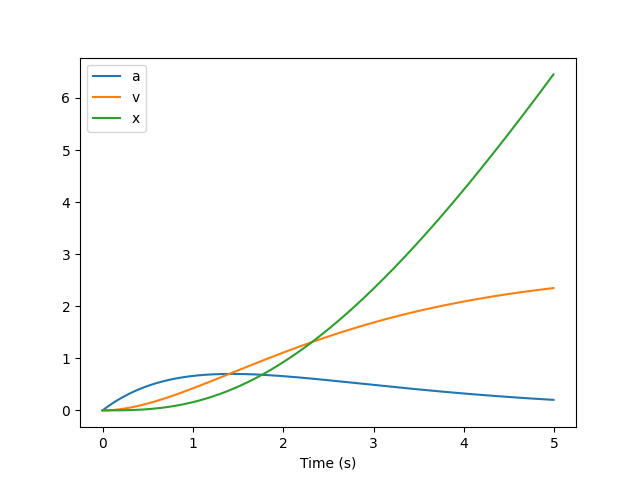
\includegraphics[scale=0.75]{Figure_1.png}
      \end{center}
\end{soln}
\newpage
% PROBLEM 4
\begin{problem}
A particle of mass $m$ moving in one dimension has potential $$U(x)=U_0\left[2\left(\frac{x}{a}\right)^2-\left(\frac{x}{a}\right)^4\right]$$ where $U_0$ and $a$ are positive constants
\end{problem}
\begin{soln} ~\\
      \begin{enumerate}[label=\alph*)]
            \item \begin{align*}
                         & F(x)=-\frac{dU(x)}{dx}                                                                               \\
                         & F(x)=-U_0\frac{d}{dx}\left[2\left(\frac{x}{a}\right)^2-\left(\frac{x}{a}\right)^4\right]             \\
                         & F(x)=-U_0\left[2\frac{d}{dx}\left(\frac{x}{a}\right)^2-\frac{d}{dx}\left(\frac{x}{a}\right)^4\right] \\
                         & F(x)=-U_0\left[\frac{4}{a}\left(\frac{x}{a}\right)-\frac{4}{a}\left(\frac{x}{a}\right)^3\right]      \\
                         & F(x)=\frac{4U_0}{a}\left[\left(\frac{x}{a}\right)^3-\left(\frac{x}{a}\right)\right]                  \\
                  \end{align*}
            \item Analytically,
                  \begin{align*}
                         & F(x)=0=\frac{4U_0}{a}\left[\left(\frac{x}{a}\right)^3-\left(\frac{x}{a}\right)\right]             \\
                         & 0 = \left(\frac{x}{a}\right)^3-\left(\frac{x}{a}\right)                                           \\
                         & 0 = \frac{x^2}{a^2}-1 \rightsquigarrow x=0 \text{ is lost here, but it is still a valid solution} \\
                         & x^2 = a^2                                                                                         \\
                         & x = \pm a \implies x=0,\pm5                                                                       \\
                  \end{align*}
                  $\pm 5$ is unstable and $0$ is stable by inspection.\\

                  Numerically (Includes code and graph for part c)),
                  \inputminted[breaklines, autogobble]{python3}{q4.py}
                  \begin{center}
                        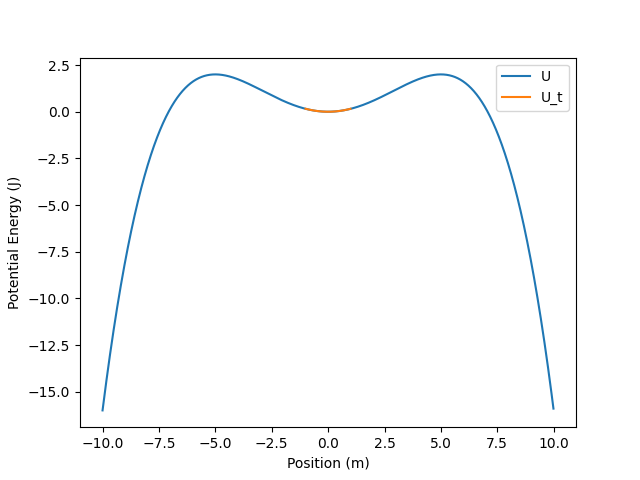
\includegraphics[scale=0.75]{Figure_2.png}
                  \end{center}
            \item $\displaystyle\sum_{n=0}^{2}\frac{f^{(n)}(x)}{n!}x^n$ So,
                  $$f(x)=U_0\left[2\left(\frac{x}{a}\right)^2-\left(\frac{x}{a}\right)^4\right]$$
                  $$f^\prime(x)=\frac{4U_0}{a}\left[\frac{x}{a}-\left(\frac{x}{a}\right)^3\right]$$
                  $$f^{\prime\prime}(x)=\frac{4U_0}{a^2}\left[1-3\left(\frac{x}{a}\right)^2\right]$$
                  Then,
                  \begin{align*}
                         & =\frac{U_0\left[2\left(\frac{x_p}{a}\right)^2-\left(\frac{x_p}{a}\right)^4\right]}{0!}x^0+\frac{\frac{4U_0}{a}\left[\frac{x_p}{a}-\left(\frac{x_p}{a}\right)^3\right]}{1!}x^1+\frac{\frac{4U_0}{a^2}\left[1-3\left(\frac{x_p}{a}\right)^2\right]}{2!}x^2 \\
                         & =\frac{2U_0}{a^2}x^2 \text{ because $x_p=0$}                                                                                                                                                                                                             \\
                  \end{align*}
                  This is still a potential and $F(x)=-\frac{dU(x)}{dx}$ holds.
                  $$\therefore F(x)=m\ddot{x}=-\frac{d}{dx}\frac{2U_0}{a^2}x^2=-\frac{4U_0}{a^2}x$$
                  Which is an equation in the form of a harmonic oscillator, which makes sense as an object with some energy placed at $x\approx 0$ would oscillate back and forth.
                  The equation can be solved to determine $x(t)$ as follows
                  \begin{align*}
                         & m\ddot{x}=-\frac{4U_0}{a^2}x\rightsquigarrow\omega_0=\sqrt{\frac{4U_0}{a^2m}} \\
                         & \ddot{x}=-\omega_0^2x                                                         \\
                         & 0=\ddot{x}+\omega_0^2x\rightsquigarrow x=e^{rt}                               \\
                         & 0=r^2e^{rt}+\omega_0^2e^{rt}                                                  \\
                         & 0=r^2+\omega_0^2                                                              \\
                         & r=\pm i\omega_0 \implies x=e^{\pm i\omega_0 t}                                \\
                  \end{align*}
                  So $x(t)=\displaystyle C_1e^{i\omega_0 t}+C_2e^{-i\omega_0 t}=C_1e^{i\sqrt{\frac{4U_0}{a^2m}} t}+C_2e^{-i\sqrt{\frac{4U_0}{a^2m}} t}$ which can be equated to
                  $(C_1+C_2)\cos(\omega_0 t)+i(C_1-C_2)\sin(\omega_0 t)=A\cos(\omega_0 t)+B\sin(\omega_0 t)$ which implies the oscillatory motion that we expect of a particle placed around the origin
            \item To escape from the origin the particle must reach either of the other points of equilibrium and fall over the side. To do this, it must have the kinetic energy equivalent (really slightly greater but only infinitesimally so)
            to the potential energy it would have at either point of unstable equilibrium ($\pm5\unit{\meter}$)
            \begin{align*}
                  & E_t=E_t^\prime\\
                  & \frac{1}{2}mv_0^2=U(\pm5) \\
                  & v_0=\sqrt{\frac{2U(\pm5)}{m}} \\
                  & v_0=\sqrt{\frac{2U_0\left[2\left(\frac{\pm5}{a}\right)^2-\left(\frac{\pm5}{a}\right)^4\right]}{m}} \\
            \end{align*}
      \end{enumerate}
\end{soln}

\end{document}